\chapter{Dizajn sustava}
\label{ch:system_design}

\selectlanguage{croatian}

\section{Arhitektura sustava}
\label{sec:architecture}

Predloženi RAG sustav temelji se na troslojnoj arhitekturi koja omogućuje skalabilnu i održivu implementaciju naprednog semantičkog pretraživanja nad EU Portalom otvorenih podataka. Arhitektura je dizajnirana prema načelima modularnosti, proširivosti i optimizacije performansi, omogućujući robusno funkcioniranje u produkcijskom okruženju.

\begin{figure}[htbp]
    \centering
    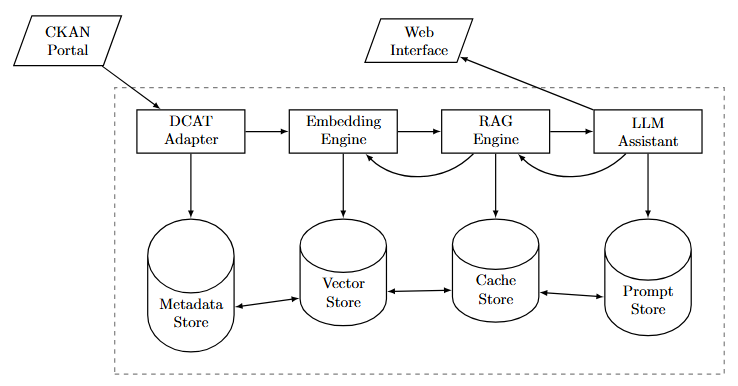
\includegraphics[width=\textwidth]{figures/system_architecture.png}
    \caption{Arhitektura sustava za analizu DCAT metapodataka}
    \label{fig:system_architecture}
\end{figure}

Sloj pohrane čini ChromaDB vektorska baza podataka koja omogućuje trajno pohranjivanje visokodimenzijskih ugradbi s optimiziranim mogućnostima pretraživanja sličnosti. Ovaj sloj također uključuje predmemoriju informacija o shemi i mehanizme predmemoriranja rezultata upita koji omogućuju značajna poboljšanja performansi za ponavljane operacije.

Sloj obrade sastoji se od Sentence Transformers modela za generiranje ugradbi, OpenAI GPT-4 integracije za generiranje SPARQL upita, te komponenti za automatsku ekstrakciju sheme koje dinamički analiziraju strukturu grafa znanja. Ovaj sloj implementira osnovnu RAG funkcionalnost kroz inteligentno dohvaćanje i procese proširenog generiranja.

Sloj sučelja omogućuje multimodalnu interakciju kroz LangChain agent okvir koji orkestrira različite strategije pretraživanja. Arhitektura temeljena na agentima omogućuje sofisticirano upravljanje tijekom rada s automatskim strategijama za vraćanje i inteligentnu sintezu rezultata kroz više izvora podataka.

\section{Ključne komponente}
\label{sec:key_components}

Sustav se sastoji od sljedećih glavnih komponenti koje implementiraju sveobuhvatnu RAG funkcionalnost. RAG System komponenta implementira osnovnu logiku povratnog dohvaćanja i generiranja kroz ChromaDB integraciju za pohranu vektora, Sentence Transformers za generiranje ugradbi, i OpenAI GPT-4 za generiranje upita. Schema Extractor komponenta automatski analizira strukturu grafa znanja EU Portala otvorenih podataka kroz ekstrakciju VoID opisa i DCAT-specifičnu analizu. Unified Data Assistant komponenta orkestrira multimodalne strategije pretraživanja kroz LangChain agent okvir koji kombinira SPARQL upite, REST API pozive i funkcionalnost API-ja za slične skupove podataka. Vektorska baza podataka komponenta omogućuje trajno pohranjivanje i učinkovito dohvaćanje semantičkih ugradbi kroz optimizirane algoritme pretraživanja sličnosti. Komponenta za validaciju upita implementira dvostupanjski proces validacije koji osigurava sintaksnu ispravnost i izvodljivost generiranih SPARQL upita. Komponenta za optimizaciju performansi implementira strategije predmemoriranja, upravljanje ograničenjima tokena i asinkrone mogućnosti obrade za optimalne performanse sustava.

\section{RAG komponente i tijek rada}
\label{sec:rag_components}

RAG sustav implementira četiri ključne komponente identificirane u istraživačkoj literaturi \cite{lewis2020retrieval, reimers2019sentence, wang2023vector}. Svaka komponenta je dizajnirana za optimalne performanse i robusno rukovanje greškama u produkcijskom okruženju.

Komponenta za ugradbe i indeksiranje koristi all-MiniLM-L6-v2 Sentence Transformers model za generiranje 384-dimenzijskih semantičkih ugradbi iz upita na prirodnom jeziku i pohranjenih primjera. ChromaDB omogućuje učinkovito pohranjivanje i dohvaćanje ovih ugradbi kroz optimizirane algoritme pretraživanja sličnosti koji koriste kosinusne metrike udaljenosti.

Komponenta za izgradnju promptova implementira sofisticiran proces sastavljanja konteksta koji kombinira dohvaćene slične primjere s relevantnim informacijama o shemi. Ovaj proces omogućuje stvaranje sveobuhvatnih promptova koji pružaju dovoljan kontekst za točno generiranje SPARQL upita dok ostaju unutar ograničenja tokena komercijalnih LLM API-ja.

Komponenta za validaciju upita implementira dvostupanjski proces validacije koji uključuje provjeru sintakse kroz parsiranje SPARQL-a i validaciju izvršavanja kroz testne upite s ograničenjima LIMIT 1. Ovaj pristup omogućuje rano otkrivanje sintaksnih grešaka i provjeru da se generirani upiti mogu uspješno izvršiti protiv ciljne krajnje točke.

\section{Multimodalni pristup pretraživanju}
\label{sec:multimodal_approach}

Unified Data Assistant implementira multimodalni pristup koji kombinira tri komplementarne strategije pretraživanja za sveobuhvatno otkrivanje skupova podataka. Ovaj pristup omogućuje optimalno pokrivanje različitih korisničkih namjera i tipova upita kroz inteligentnu orkestraciju više metoda pristupa podacima.

RAG-prošireno generiranje SPARQL upita predstavlja primarnu strategiju pretraživanja koja koristi semantičko pretraživanje sličnosti za dohvaćanje relevantnih primjera upita i informacija o shemi. Ovaj pristup je optimiziran za strukturirane upite koji zahtijevaju precizno filtriranje i složena spajanja kroz više svojstava skupova podataka.

REST API pretraživanje omogućuje fleksibilno pretraživanje temeljeno na ključnim riječima s mogućnostima facetiranja preko izdavača, formata, teme i vremenskih dimenzija. Ovaj pristup je idealan za istraživačke upite gdje korisnici nisu sigurni o točnoj terminologiji ili strukturi ciljnih skupova podataka.

API za slične skupove podataka koristi vlastite algoritme platforme sličnosti za otkrivanje povezanih skupova podataka na temelju sličnosti metapodataka. Ovaj pristup omogućuje neočekivano otkrivanje povezanih skupova podataka koji možda nisu odmah očigledni kroz tradicionalne metode pretraživanja.

\section{Ekstrakcija sheme i analiza grafa znanja}
\label{sec:schema_extraction}

Sustav za automatsku ekstrakciju sheme implementira sveobuhvatnu analizu strukture grafa znanja EU Portala otvorenih podataka kroz kombinaciju ekstrakcije VoID opisa i DCAT-specifične analize. Ovaj sustav omogućuje dinamičko razumijevanje strukture skupa podataka i uzoraka korištenja rječnika koji su bitni za informirano generiranje upita.

Komponenta za ekstrakciju VoID opisa automatski dohvaća sveobuhvatne statistike o strukturi grafa znanja uključujući ukupan broj trojki, različitih subjekata, klasa i svojstava. Ove informacije omogućuju razumijevanje opsega i složenosti ciljnog grafa znanja što je ključno za optimizaciju strategija generiranja upita.

DCAT-specifična analiza fokusira se na ekstrakciju domenski specifičnih statistika relevantnih za ekosustav EU Portala otvorenih podataka. Analiza uključuje nabrajanje broja skupova podataka, formata distribucije, statistika izdavača, pokrivanje tema i vremenske uzorke koji omogućuju specijaliziranu optimizaciju za kontekst europskih otvorenih podataka.

Nabrajanje klasa i svojstava sa statistikama korištenja omogućuje identifikaciju najčešće korištenih pojmova rječnika i njihovih odnosa unutar grafa znanja. Ova informacija je integrirana u proces izgradnje RAG promptova za generiranje upita koji slijede ustaljene uzorke i koriste odgovarajuće pojmove rječnika.

\section{Orkestracija temeljena na agentima}
\label{sec:agent_orchestration}

LangChain agent okvir omogućuje sofisticiranu orkestraciju više strategija pretraživanja kroz inteligentno upravljanje tijekom rada. Arhitektura temeljena na agentima implementira logiku donošenja odluka koja određuje optimalnu strategiju pretraživanja na temelju karakteristika upita, korisničke namjere i dostupnih resursa.

Inženjerstvo agent promptova implementira sveobuhvatne upute koje vode ponašanje agenta kroz složene višestupanjske tokove rada. Promptovi su dizajnirani da potiču sistemski pristup koji počinje s RAG-proširenim generiranjem SPARQL upita, nastavlja kroz API pretraživanja, i završava s inteligentnom sintezom i analizom rezultata.

Integracija alata omogućuje besprijekorna interakcija između različitih komponenti pretraživanja kroz standardizirana sučelja. Svaki alat implementira robusno rukovanje greškama i pruža strukturirani izlaz koji može biti lako obrađen od strane logike donošenja odluka agenta.

Komponenta za sintezu rezultata implementira inteligentnu analizu i kombinaciju rezultata iz više strategija pretraživanja. Ovaj proces uključuje uklanjanje duplikata, rangiranje relevantnosti, i sveobuhvatno sažimanje koje korisnicima pruža praktične uvide o dostupnim skupovima podataka.

\section{Strategije optimizacije performansi}
\label{sec:performance_optimization}

Optimizacija performansi u RAG sustavu implementirana je kroz predmemoriranje na više razina, inteligentno upravljanje resursima i optimizirane strukture podataka. Ove strategije omogućuju vremena odgovora u sekundama za pretraživanja sličnosti i razumna vremena odgovora za složene multimodalne upite.

Optimizacija vektorskog pretraživanja implementirana je kroz ChromaDB trajno pohranjivanje koje omogućuje brzo pokretanje sustava i dosljedne performanse kroz sesije. Operacije u skupinama i optimizirane strategije indeksiranja omogućuju učinkovito rukovanje velikim kolekcijama primjera upita bez značajne degradacije performansi.

Upravljanje ograničenjima tokena implementirano je kroz inteligentne strategije skraćivanja koje čuvaju najvažnije informacije dok ostaju unutar ograničenja komercijalnih API-ja. Tehnike sažimanja rezultata i kompresije konteksta omogućuju učinkovito rukovanje velikim skupovima rezultata bez gubitka kritičnih informacija.

Asinkrone mogućnosti obrade omogućuju paralelno izvršavanje više strategija pretraživanja što rezultira bržim ukupnim vremenima odgovora. Strategije predmemoriranja na više razina uključujući predmemoriju ugradbi, predmemoriju sheme i predmemoriju rezultata omogućuju značajna poboljšanja performansi za ponavljane upite.

\section{Rukovanje greškama i robusnost}
\label{sec:error_handling}

Sveobuhvatno rukovanje greškama implementirano je kroz više slojeva sustava za osiguravanje robusnog funkcioniranja u produkcijskom okruženju. Strategije rukovanja greškama uključuju graciozan pad, automatske mehanizme ponovnog pokušaja i sveobuhvatno bilježenje za otklanjanje grešaka i nadzor.

Validacija SPARQL upita implementira dvostupanjski pristup koji hvata sintaksne greške prije izvršavanja i pruža značajne poruke o greškama za otklanjanje grešaka. Automatski mehanizmi ponovnog pokušaja s profinjavanjem konteksta omogućuju oporavak od privremenih kvarova i poboljšanje kvalitete upita kroz iterativno pročišćavanje.

Rukovanje API greškama implementira robusne strategije za rukovanje ograničenjima brzine, vremenskim ograničenjima mreže i nedostupnosti servisa. Rezervni mehanizmi omogućuju nastavak rada čak i kada pojedinačne komponente nisu dostupne, osiguravajući dosljedno korisničko iskustvo.

Bilježenje i nadzor implementirani su kroz sveobuhvatan okvir koji prati metrike performansi, stope grešaka i uzorke korisničkih interakcija. Ove informacije omogućuju kontinuirano poboljšanje sustava i proaktivnu identifikaciju potencijalnih problema prije nego što utječu na korisničko iskustvo.

\section{Skalabilnost i razmatranja za implementaciju}
\label{sec:scalability}

Sustav je dizajniran za horizontalno skaliranje kroz modularnu arhitekturu i dizajn komponenti bez stanja. ChromaDB trajno pohranjivanje omogućuje jednostavne strategije sigurnosnog kopiranja i migracije, dok kontejnerizirano implementiranje omogućuje fleksibilnu dodjelu resursa i skaliranje na temelju potražnje.

Upravljanje resursima implementirano je kroz inteligentne strategije dodjele koje uravnotežuju točnost i performanse na temelju dostupnih računalnih resursa. Prilagodljivi algoritmi omogućuju automatsko prilagođavanje parametara obrade na temelju opterećenja sustava i zahtjeva za vremenom odgovora.

Upravljanje konfiguracije omogućuje jednostavno prilagođavanje sustava za različita okruženja implementacije i slučajeve korištenja. Parametrizirane komponente omogućuju fino podešavanje karakteristika performansi bez potrebe za izmjenama koda, omogućujući optimalno funkcioniranje u različitim produkcijskim scenarijima. 